\documentclass[12pt]{article}
\usepackage{graphicx} % Required for inserting images
\usepackage{mathtools}
\usepackage{amsmath}
\usepackage{gvv-book}
\usepackage{gvv}
\usepackage[shortlabels]{enumitem}
\usepackage{multicol}

\title{\textbf{12.18}}
\author{\textbf{EE25BTECH11004 - Aditya Appana}}
\date{October 5, 2025}
\renewcommand{\labelenumi}{\Alph{enumi})}
\begin{document}

\maketitle

\section*{Question}
$\vec{X}$ is 1 km northeast of $\vec{Y}$. $\vec{Y}$ is 1 km southeast of $\vec{Z}$. $\vec{W}$ is 1 km west of $\vec{Z}$. $\vec{P}$ is 1
km south of $\vec{W}$. $\vec{Q}$ is 1 km east of $\vec{P}$. What is the distance between $\vec{X}$ and $\vec{Q}$ in km?
\begin{enumerate}
\begin{multicols}{4}
    \item 1
    \item $\sqrt{2}$
    \item $\sqrt{3}$
    \item 2
\end{multicols}
\end{enumerate}
\section*{Solution}

Let $\vec{X}$ be $\myvec{0\\0}$. Every subsequent vector can be expressed as a translation by a unit vector, from the previous vector. The translation vector can be represented as:\\
\begin{align}
\myvec{\cos\theta \\ \sin\theta}
\end{align}
\end{frame}

$\vec{X}$ is 1km north-east of $\vec{Y}$, so $\vec{Y}$ is 1km south-west of $\vec{X}$. Therefore:\begin{align}
\vec{Y}-\vec{X} = \myvec{\cos225\degree \\ \sin225\degree}\\
\vec{Y}-\vec{X} = \myvec{\frac{-1}{\sqrt{2}}\\\frac{-1}{\sqrt{2}}}
\end{align}\\
$\vec{Y}$ is 1km south-east of $\vec{Z}$, so $\vec{Z}$ is 1km north-west of $\vec{Y}$. Therefore:\begin{align}
\vec{Z}-\vec{Y} = \myvec{\cos135\degree \\ \sin135\degree}\\
\vec{Z}-\vec{Y} = \myvec{\frac{-1}{\sqrt{2}}\\\frac{1}{\sqrt{2}}}
\end{align}\\
$\vec{W}$ is 1km west of $\vec{Z}$. Therefore:\begin{align}
\vec{W}-\vec{Z} = \myvec{\cos180\degree \\ \sin180\degree}\\
\vec{W}-\vec{Z} = \myvec{-1\\0}
\end{align}\\
$\vec{P}$ is 1km south of $\vec{W}$. Therefore:\begin{align}
\vec{P}-\vec{W} = \myvec{\cos270\degree \\  \cos270\degree}\\
\vec{P}-\vec{W} = \myvec{0\\-1}
\end{align}\\
$\vec{Q}$ is 1km east of $\vec{P}$. Therefore:\begin{align}
\vec{Q}-\vec{P} = \myvec{\cos0\degree \\ \sin0\degree}\\
\vec{Q}-\vec{P} = \myvec{1\\0}
\end{align}\\
Adding (3), (5), (7), (9), (11) together, we get $\vec{Q}-\vec{X} =\vec{Q} = \myvec{-\sqrt{2}\\-1}$.\\
The distance between $\vec{X}=\myvec{0\\0}$ and $\vec{Q}=\myvec{-\sqrt{2}\\-1}$ is:
\begin{align}
    ||\vec{X} - \vec{Q}||= \norm{\myvec{\sqrt{2}\\1}} \\
    \sqrt{(\sqrt{2})^2 +1^2} = \sqrt{3}
\end{align}\\
Therefore the correct option is \textbf{C}.


\begin{figure}[H]
    \centering
    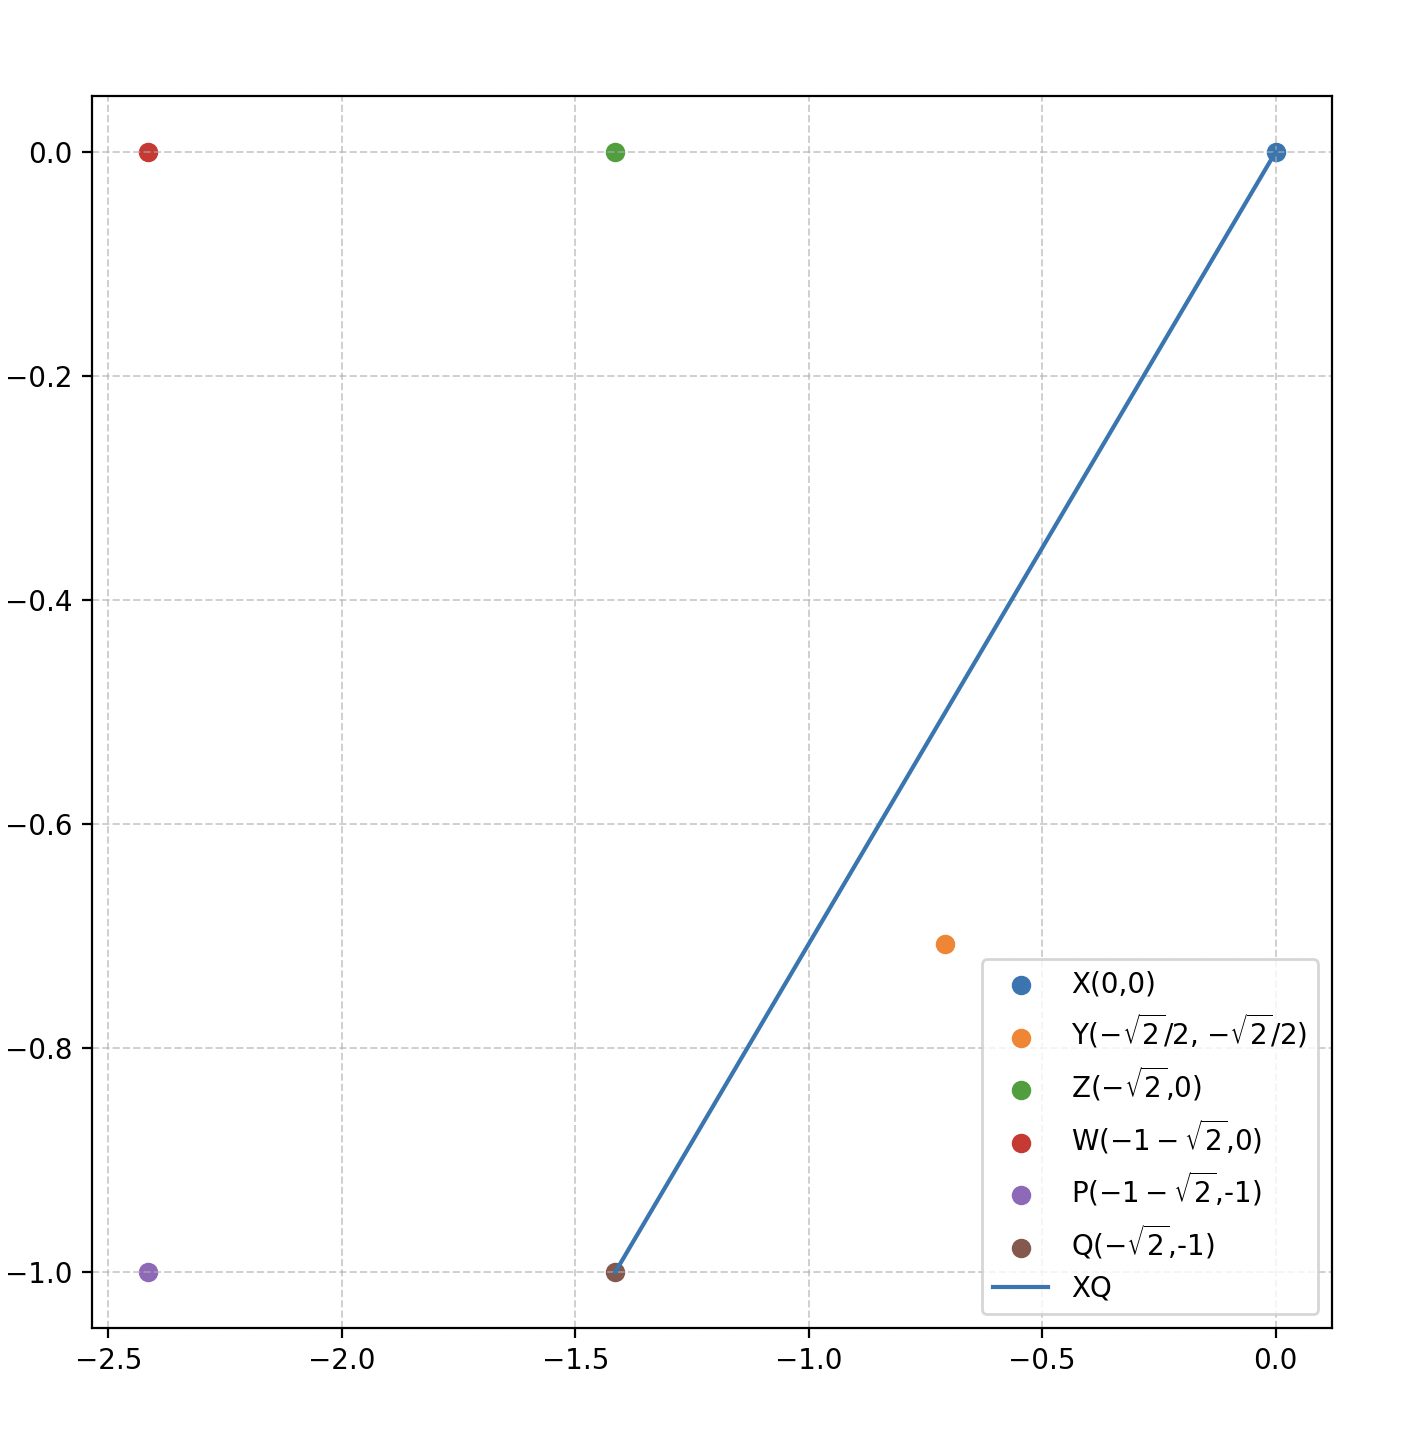
\includegraphics[width=0.8\columnwidth]{Figs/1218.png}
    \caption{Plot}
    \label{fig:placeholder}
\end{figure}
\end{document}
